\chapter{Análisis económico}\label{chapter04}

\section{Modelo de negocio}

El modelo de negocio de AIVA se orienta a ofrecer a comercios de alimentos perecederos una plataforma web que pronostica la demanda diaria por producto y habilita decisiones operativas basadas en datos. La propuesta enfatiza un costo total de propiedad acotado, tiempos de respuesta breves y explicabilidad de los resultados, de modo que cada recomendación pueda ser auditada y comprendida por el equipo del local. El enfoque prioriza el impacto económico directo mediante la reducción de mermas y quiebres de stock, la mejora de la rotación y un ahorro de tiempo en tareas de carga y análisis.

Con el objetivo de representar de manera estructurada la lógica de creación, entrega y captura de valor de la solución, se adopta como marco el \textit{Business Model Canvas} (BMC). Esta herramienta permite describir y analizar de forma sistemática los distintos componentes del modelo de negocio —propuesta de valor, clientes, canales, recursos, actividades, socios, estructura de costos e ingresos— y constituye la base conceptual que habilita posteriormente el desarrollo del análisis financiero. De este modo, el BMC actúa como puente entre la definición estratégica del proyecto y la evaluación cuantitativa de su viabilidad económica.

\subsection{Propuesta de Valor}
AIVA propone una plataforma web de fácil adopción para comercios que operan con productos perecederos (panaderías, confiterías y tiendas naturales), orientada a reducir mermas y faltantes mediante planificación basada en datos. La solución integra modelos de predicción de demanda con series temporales y variables exógenas (clima y feriados), un asistente conversacional para consultas operativas y un flujo de carga asistida por imágenes (OCR) que minimiza la fricción de ingreso de datos. El valor se manifiesta en una mejora de la disponibilidad de productos, una disminución del desperdicio y una optimización de los recursos de producción, traduciéndose en mayor eficiencia operativa y márgenes más saludables para el comerciante.

\subsection{Segmentos de Clientes}
El segmento objetivo está conformado por pequeñas y medianas empresas del sector de alimentos perecederos, con foco en panaderías y confiterías de barrio. Se trata de negocios con recursos limitados para soluciones corporativas complejas, pero con necesidad crítica de herramientas predictivas que acompañen decisiones diarias de producción y reposición.
En esta primera etapa de desarrollo, el proyecto se plantea como meta alcanzar un parque de mil usuarios activos, conformado por comercios de pequeña y mediana escala dentro del sector de alimentos perecederos. Esta cifra funciona como horizonte de referencia tanto para dimensionar la infraestructura tecnológica como para proyectar el análisis financiero del modelo de negocio.

\subsection{Canales}
La captación se apoya primordialmente en publicidad digital, para la cual se asigna el 50\% del valor de la suscripción (USD~15 por usuario activo). Este canal permite adquisición directa, medible y escalable. La estrategia se complementa con difusión orgánica (boca a boca) y presencia sectorial, a efectos de reforzar la marca en el ámbito de referencia del cliente objetivo.

\subsection{Relación con los Clientes}
El modelo de relación combina autoservicio digital para el registro y uso inicial con soporte técnico y funcional por correo electrónico. Este esquema preserva la escalabilidad sin desatender la asistencia necesaria durante la adopción y operación, especialmente en etapas de onboarding y calibración del modelo predictivo.

\subsection{Recursos Clave}
Los recursos críticos son la infraestructura y las capacidades analíticas. En backend, \emph{Supabase Pro} ofrece hasta 100{,}000 usuarios activos mensuales incluidos, 250~GB/mes de egress (con amplio margen frente al patrón de uso de 1{,}000 usuarios) y 8~GB de base de datos (con ampliación bajo demanda), además de 100~GB de almacenamiento. En frontend, \emph{Vercel Pro} proporciona despliegue continuo, edge network, caché y observabilidad, suficientes para garantizar disponibilidad y rendimiento frente a la meta de 1{,}000 usuarios. A ello se suman APIs de terceros: datos meteorológicos (OpenWeather), capacidades de reconocimiento óptico de caracteres (OCR) y modelos de lenguaje de gran escala provistos por OpenAI, que sustentan tanto el asistente conversacional como los procesos de interpretación de datos visuales. Estos recursos tecnológicos fortalecen la diferenciación funcional de AIVA y garantizan una experiencia de usuario fluida, explicable y de alto valor agregado.

\subsection{Actividades Clave}
Las actividades esenciales incluyen el desarrollo y mantenimiento de la plataforma, la mejora continua de los modelos de predicción (monitoreo de error y recalibración), la operación y observabilidad del servicio en producción, la ejecución de campañas de adquisición digital y la provisión de soporte al usuario final. La consistencia entre predicción y operación diaria del comercio es un objetivo permanente.

\subsection{Socios Clave}
Si bien la adquisición es directa, se consideran aliados sectoriales (cámaras de panaderos y confiterías) para facilitar el acceso al mercado objetivo y la validación funcional. En lo tecnológico, los proveedores de nube y APIs (Supabase, Vercel, OpenAI y clima) constituyen socios clave que habilitan escalabilidad, confiabilidad y rapidez de iteración.

\subsection{Estructura de Costos}
La estructura combina costos fijos y variables. Entre los fijos se contemplan las suscripciones de infraestructura (Supabase Pro y Vercel Pro) y las herramientas de operación. Entre los variables se incluyen publicidad digital (USD~15 por usuario activo al mes asignados a adquisición), uso incremental de APIs (LLM, OCR, clima), almacenamiento y egress por encima de los tramos incluidos, y el soporte operativo. Adicionalmente, cada alta entra en un período de prueba de un mes, durante el cual los costos recaen sobre AIVA sin ingresos asociados, por lo que representa un costo directo de adquisición. La inversión inicial (CapEx) en desarrollo e ingeniería se registra previo al lanzamiento del servicio.

\subsection{Fuentes de Ingresos}
El ingreso proviene de una suscripción mensual de USD~30 por usuario. Este flujo recurrente se modela con una tasa de cancelación (churn) mensual del 5\%, incorporando además la conversión del período de prueba (trial) al plan pago. La combinación de suscripción, retención y adquisición digital permite proyectar escalabilidad de ingresos acorde con el crecimiento del parque de clientes.

\subsection{Indicadores Financieros Clave}
Para evaluar la sostenibilidad económica del modelo se incorporan métricas estándar de negocios por suscripción.

\paragraph{Costo de Adquisición de Cliente (CAC).}
Sea $G$ el gasto de adquisición por alta y $\gamma$ la tasa de conversión de \emph{trial} a pago. El CAC se define como
\[
CAC \;=\; \frac{G}{\gamma}.
\]
Dado $G = \text{USD }15$ (50\% de la suscripción asignado a publicidad) y $\gamma = 0{,}42$, se obtiene
\[
CAC \;=\; \frac{15}{0{,}42} \approx \text{USD }35{,}7.
\]

\paragraph{Valor de Vida del Cliente (LTV).}
Con un ingreso medio por usuario (ARPU) igual al precio mensual del plan y $c$ como churn mensual, el LTV se aproxima como
\[
LTV \;=\; \frac{ARPU}{c}.
\]
Bajo $ARPU = \text{USD }30$ y $c = 0{,}05$, resulta
\[
LTV \;=\; \frac{30}{0{,}05} \;=\; \text{USD }600.
\]

\paragraph{Relación LTV/CAC.}
La razón $LTV/CAC$ sintetiza la eficiencia de adquisición:
\[
\frac{LTV}{CAC} \;=\; \frac{600}{35{,}7} \;\approx\; 16{,}8.
\]
En términos de buenas prácticas SaaS, valores superiores a 3 son deseables; el presente resultado indica un margen holgado para sostener inversión en marketing y acciones de retención sin comprometer la rentabilidad.



\section{Análisis financiero}

\subsection{Metodología}

El modelo financiero se estructura sobre un servicio por suscripción mensual de USD~30 con un mes de prueba inicial sin cargo. La inclusión de un período de prueba se fundamenta en evidencia empírica que demuestra cómo el diseño de los \textit{trials} puede incidir en la adopción y la conversión: estudios experimentales en plataformas SaaS confirman que extender o personalizar la duración de la prueba incrementa tanto su utilización como la probabilidad de que los usuarios se conviertan en clientes pagos (Zhang, 2025). En este marco, se adopta una tasa de conversión post‐trial del 42\% como supuesto de referencia, entendida como una hipótesis informada por la literatura, que posteriormente deberá ser contrastada con datos reales de operación.

En cuanto a la tasa de cancelación (\textit{churn}), los benchmarks de referencia para SaaS B2B muestran que, en servicios con un precio mensual entre USD~25 y USD~50, el churn promedio es de 7,3\% (Vitally, 2025). En este análisis se adopta un 6\% como supuesto operativo, lo que representa una postura conservadora que evita sobredimensionar la retención de usuarios.



La sostenibilidad del modelo se evalúa mediante métricas propias de negocios por suscripción: el costo de adquisición de cliente (CAC), el valor de vida del cliente (LTV) y la razón entre ambos indicadores. Estas métricas constituyen estándares de análisis en la literatura aplicada y en la práctica de evaluación de startups, ya que permiten determinar si los ingresos generados por cada cliente a lo largo de su permanencia superan ampliamente los costos de captación (Burkland Finance, 2024). A partir de estos supuestos, se construye un escenario base que constituye la referencia principal del análisis financiero. Sobre esta base, y modificando parámetros clave como la tasa de crecimiento, se elaboran los escenarios pesimista y optimista, lo que permite evaluar la sensibilidad del modelo frente a diferentes condiciones de mercado.



\subsection{Estructura de costos: CapEx}
La inversión inicial (\emph{CapEx}) corresponde principalmente a recursos humanos para el desarrollo del MVP y el despliegue productivo. Se contemplan seis roles, con tarifas medias y dedicación acumulada de seis meses (o equivalentes). El detalle se presenta en la Figura~\ref{fig:capex}.

\begin{figure}[!htbp]
  \centering
  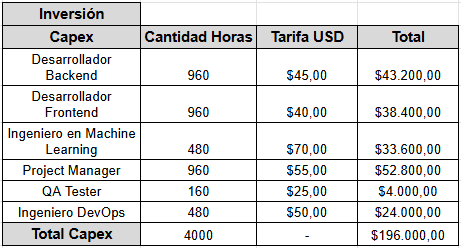
\includegraphics[width=0.85\textwidth]{images/Capex.PNG}
  \caption{Detalle de CapEx por rol -- Fuente: elaboración propia}
  \label{fig:capex}
\end{figure}

\subsection{Estructura de costos: OpEx}
El \emph{OpEx} mensual combina componentes fijos y variables. Entre los fijos se incluyen hosting del frontend y base de datos/backend; entre los variables: publicidad proporcional a las altas, impuestos locales sobre ingresos brutos, comisiones de facturación/cobranza, uso de tokens de OpenAI y servicios de clima. La Figura~\ref{fig:costos-variables-fijas} resume los parámetros fijos empleados en el modelo.

\begin{figure}[!htbp]
  \centering
  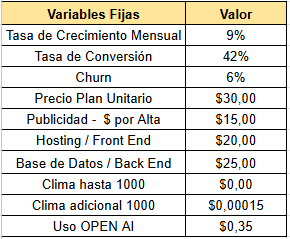
\includegraphics[width=0.6\textwidth]{images/CostosVariablesFijas.PNG}
  \caption{Variables fijas para costos -- Fuente: elaboración propia}
  \label{fig:costos-variables-fijas}
\end{figure}

El detalle mensual del OpEx se presenta en las Figuras~\ref{fig:opex-anio1}, \ref{fig:opex-anio2} y \ref{fig:opex-anio3}, correspondientes a los tres primeros años de operación.

\begin{figure}[!htbp]
  \centering
  \includegraphics[width=0.92\textwidth]{images/OpexAño1.PNG}
  \caption{OpEx mensual, Año 1 -- Fuente: elaboración propia}
  \label{fig:opex-anio1}
\end{figure}

\begin{figure}[!htbp]
  \centering
  \includegraphics[width=0.92\textwidth]{images/OpexAño2.PNG}
  \caption{OpEx mensual, Año 2 -- Fuente: elaboración propia}
  \label{fig:opex-anio2}
\end{figure}

\begin{figure}[!htbp]
  \centering
  \includegraphics[width=0.92\textwidth]{images/OpexAño3.PNG}
  \caption{OpEx mensual, Año 3 -- Fuente: elaboración propia}
  \label{fig:opex-anio3}
\end{figure}


\subsection{Ingresos y dinámica de conversión}

En el escenario base del modelo financiero se adopta una tasa de crecimiento mensual de altas del 9\%. Este parámetro se encuentra alineado con los rangos reportados para startups de software como servicio (SaaS) en fases iniciales, donde la literatura especializada identifica tasas de expansión mensual de entre 5\% y 10\% como habituales en etapas de tracción temprana (Burkland Finance, 2024). Bajo este supuesto, los ingresos se reconocen exclusivamente por clientes pagos, es decir, aquellos que han atravesado el período de prueba y se han convertido efectivamente en suscriptores.

En cuanto a los costos variables asociados al uso de inteligencia artificial, el análisis estima un cargo aproximado de USD~0,35 por usuario activo mensual correspondiente a consultas a modelos de OpenAI (tanto para el asistente conversacional como para funciones de OCR). Este valor surge de proyectar el patrón de uso definido en el caso base (alrededor de 30 consultas diarias por usuario, con una media de tokens por interacción y las tarifas vigentes de la API), lo que permite dimensionar de manera realista el impacto unitario de la infraestructura cognitiva sobre el costo operativo.

Finalmente, los resultados consolidados permiten sintetizar los principales indicadores financieros del escenario base. En el horizonte de tres años, los ingresos acumulados alcanzan aproximadamente USD~929.270, mientras que los costos operativos totales (OPEX) ascienden a USD~313.841. La inversión inicial (CapEx), correspondiente al desarrollo de la plataforma y adquisición de equipamiento, se sitúa en USD~196.000 adicionales. Este resumen evidencia que, bajo los supuestos planteados, el modelo proyecta una senda de crecimiento sostenible en la que los ingresos superan ampliamente los costos, validando la viabilidad económica de la propuesta.


\begin{figure}[!htbp]
  \centering
  \includegraphics[width=0.92\textwidth]{images/CashflowAño1.PNG}
  \caption{Cashflow proyectado, Año 1 -- Fuente: elaboración propia}
  \label{fig:cashflow-anio1}
\end{figure}

\begin{figure}[!htbp]
  \centering
  \includegraphics[width=0.92\textwidth]{images/CashflowAño2.PNG}
  \caption{Cashflow proyectado, Año 2 -- Fuente: elaboración propia}
  \label{fig:cashflow-anio2}
\end{figure}

\begin{figure}[!htbp]
  \centering
  \includegraphics[width=0.92\textwidth]{images/CashflowAño3.PNG}
  \caption{Cashflow proyectado, Año 3 -- Fuente: elaboración propia}
  \label{fig:cashflow-anio3}
\end{figure}


\subsection{Flujo de fondos del caso base}

El flujo de fondos proyectado para el caso base integra los ingresos por suscripciones, los costos operativos (OPEX) y la inversión inicial en desarrollo y equipamiento (CapEx). La dinámica se construye sobre el supuesto de crecimiento mensual del 9\% en altas de usuarios, con una conversión del 42\% post--trial, una tasa de cancelación mensual del 6\% y una tasa anual del 20\% que se utiliza en los 3 escenarios propuestos. 

En el \textbf{Año 1}, los ingresos generados resultan todavía insuficientes para cubrir la inversión inicial y los costos operativos, lo que mantiene el flujo acumulado en valores negativos a lo largo de los primeros meses. A medida que avanza el año, la curva de ingresos se acelera y reduce progresivamente el déficit acumulado, pasando de --USD~196.000 en el inicio a --USD~170.845 al cierre del mes 12.  

Durante el \textbf{Año 2}, la progresión de clientes pagos permite un crecimiento sostenido en los ingresos. Este efecto acelera la reducción del déficit acumulado, que desciende desde --USD~164.618 en el mes 13 hasta --USD~25.475 al finalizar el mes 24. El negocio se aproxima al punto de equilibrio financiero (\textit{break-even}), el cual se alcanza en el transcurso del tercer año.  

Finalmente, en el \textbf{Año 3}, el flujo acumulado se torna positivo y refleja un proceso de recuperación de la inversión inicial. A partir del mes 27 se alcanza el \textit{break-even} (USD~45.744 acumulados), y desde allí los excedentes se amplían con rapidez hasta llegar a un saldo positivo de USD~419.427 al cierre del mes 36. Este comportamiento confirma la viabilidad económica del modelo bajo los parámetros establecidos en el escenario base.  

Las Figuras~\ref{fig:flujo-anio1}, \ref{fig:flujo-anio2} y \ref{fig:flujo-anio3} muestran en detalle la evolución mensual del flujo de fondos para cada uno de los tres años analizados.

\begin{figure}[!htbp]
  \centering
  \includegraphics[width=0.95\textwidth]{images/FlujodefondosAño1.PNG}
  \caption{Flujo de fondos proyectado -- Año 1. Fuente: elaboración propia}
  \label{fig:flujo-anio1}
\end{figure}

\begin{figure}[!htbp]
  \centering
  \includegraphics[width=0.95\textwidth]{images/FlujodefondosAño2.PNG}
  \caption{Flujo de fondos proyectado -- Año 2. Fuente: elaboración propia}
  \label{fig:flujo-anio2}
\end{figure}

\begin{figure}[!htbp]
  \centering
  \includegraphics[width=0.95\textwidth]{images/FlujodefondosAño3.PNG}
  \caption{Flujo de fondos proyectado -- Año 3. Fuente: elaboración propia}
  \label{fig:flujo-anio3}
\end{figure}



\subsection{Análisis comparativo de escenarios}

Con el objetivo de evaluar la robustez del modelo financiero se plantearon tres escenarios de crecimiento: pesimista (5\%), base (9\%) y optimista (12\%). Antes de examinar sus resultados, se definen brevemente los principales indicadores utilizados en la comparación:

\begin{itemize}
  \item \textbf{Valor Actual Neto (VAN)}: mide la diferencia entre los flujos de caja futuros descontados a una tasa determinada y la inversión inicial. Un VAN positivo indica que el proyecto genera valor económico sobre el costo de capital.
  \item \textbf{Tasa Interna de Retorno (TIR)}: representa la tasa de descuento que iguala a cero el VAN. Es decir, la rentabilidad implícita del proyecto. Cuanto mayor sea la TIR respecto al costo de capital, más atractivo es el emprendimiento.
  \item \textbf{Payback}: señala el tiempo requerido para recuperar la inversión inicial a través de los flujos netos de caja. A menor período de recuperación, menor es el riesgo financiero.
\end{itemize}

\paragraph{Escenario pesimista (5\% de crecimiento mensual).}  
En esta proyección el modelo alcanza ingresos acumulados por USD~463.716 al cabo de tres años, con un OPEX total de USD~140.543. El VAN resulta positivo, aunque reducido (USD~15.531), mientras que la TIR se ubica en 24\%. El período de repago de la inversión inicial se extiende a 2 años y 6 meses. Este escenario refleja que, aun con un ritmo bajo de crecimiento, la propuesta mantiene viabilidad económica, pero con márgenes ajustados y retornos moderados.

\paragraph{Escenario base (9\% de crecimiento mensual).}  
Se trata del caso central de análisis. Bajo estos parámetros los ingresos totales ascienden a USD~929.270 en tres años, con un OPEX acumulado de USD~313.842. El VAN se eleva a USD~191.940 y la TIR alcanza un 53\%. El payback se logra en 2 años y 2 meses. Este escenario confirma que, con una dinámica de crecimiento acorde a benchmarks de SaaS en etapas iniciales, el modelo no solo cubre con holgura la inversión inicial de USD~196.000, sino que además genera una rentabilidad significativa.

\paragraph{Escenario optimista (12\% de crecimiento mensual).}  
Bajo un desempeño más acelerado, los ingresos totales alcanzan USD~1.643.576 en el período analizado, con un OPEX proporcionalmente mayor (USD~605.135). El VAN asciende a USD~443.576 y la TIR alcanza el 75\%. El payback se produce en apenas 2 años. Este resultado muestra el potencial de escalabilidad del modelo: una mayor tracción comercial acelera la recuperación de la inversión y multiplica el valor económico generado.

\paragraph{Comparación y conclusiones.}  
El contraste entre los tres escenarios permite observar la sensibilidad del modelo a la tasa de crecimiento mensual de usuarios. Mientras que con un 5\% el proyecto mantiene apenas la viabilidad financiera, a partir del 9\% se consolida como rentable y sostenible, y con un 12\% despliega un perfil altamente atractivo para inversionistas. Esto confirma que la variable crítica del modelo no reside únicamente en los costos fijos o variables, sino en la capacidad de sostener un ritmo de crecimiento en la base de clientes que garantice retornos adecuados sobre la inversión.


\begin{figure}[!htbp]
  \centering
  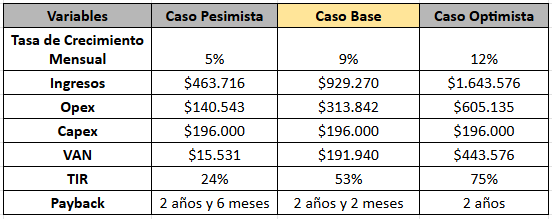
\includegraphics[width=0.9\textwidth]{images/AnalisisFinal.PNG}
  \caption{Comparación de escenarios: pesimista, base y optimista. Fuente: elaboración propia}
  \label{fig:analisis-final}
\end{figure}